\documentclass[12pt]{article}
\usepackage[margin=0.8in]{geometry}
\usepackage{booktabs}
\usepackage{multirow}
\usepackage{graphicx}
\usepackage{array}
\usepackage{xcolor}
\usepackage{colortbl}
\usepackage{adjustbox}

\begin{document}

% Table 1: Comprehensive table with statistics and examples
\begin{table}[htbp]
\centering
\caption{Reconstruction Error and Accuracy by ROI and Group with Representative Examples}
\label{tab:reconstruction_with_examples}
\small
\setlength{\tabcolsep}{5pt}
\renewcommand{\arraystretch}{1.5}
\begin{tabular}{|c|c|c|c|c|}
\hline
\rowcolor{blue!30}
\textbf{ROI} & \textbf{Group} & \textbf{Mean Error} & \textbf{Acc@45° (\%)} & \textbf{Example} \\
\hline
\hline
\multirow{2}{*}{\textbf{V1}} & \textbf{HC} & 46.7° (SD 17.0°) & 59.6 (SD 25.1) & \adjustbox{valign=c}{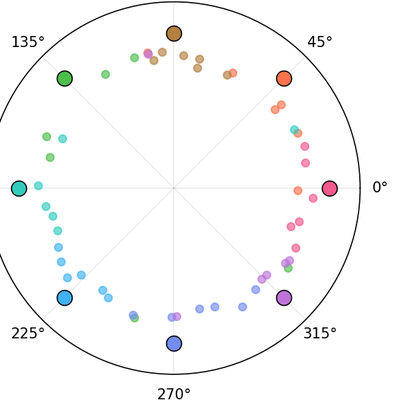
\includegraphics[width=2.5cm,height=2.5cm]{cropped_clean/clean_noncvd_V1.png}} \\
\cline{2-5}
 & \textbf{CVD} & 42.4° (SD 4.9°) & 67.6 (SD 18.0) & \adjustbox{valign=c}{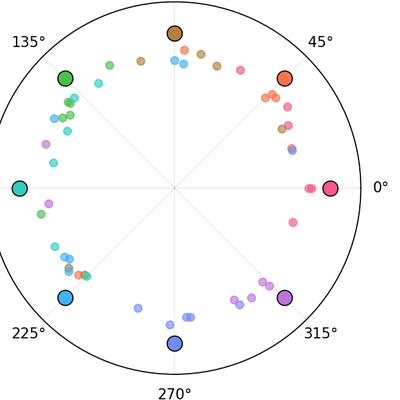
\includegraphics[width=2.5cm,height=2.5cm]{cropped_clean/clean_cvd_V1.png}} \\
\hline
\multirow{2}{*}{\textbf{V2}} & \textbf{HC} & 56.9° (SD 16.8°) & 50.0 (SD 21.8) & \adjustbox{valign=c}{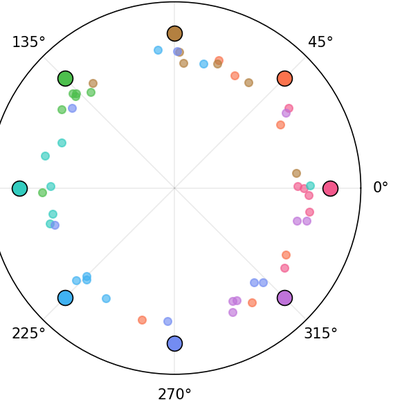
\includegraphics[width=2.5cm,height=2.5cm]{cropped_clean/clean_noncvd_V2.png}} \\
\cline{2-5}
 & \textbf{CVD} & 55.3° (SD 5.1°) & 40.9 (SD 3.8) & \adjustbox{valign=c}{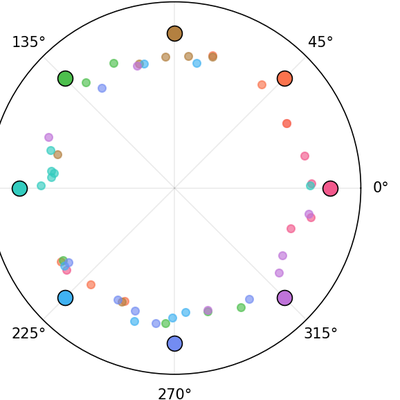
\includegraphics[width=2.5cm,height=2.5cm]{cropped_clean/clean_cvd_V2.png}} \\
\hline
\multirow{2}{*}{\textbf{V3}} & \textbf{HC} & 82.8° (SD 14.1°) & 27.9 (SD 5.1) & \adjustbox{valign=c}{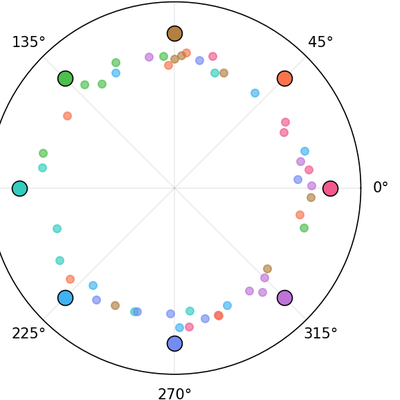
\includegraphics[width=2.5cm,height=2.5cm]{cropped_clean/clean_noncvd_V3.png}} \\
\cline{2-5}
 & \textbf{CVD} & 78.9° (SD 7.5°) & 28.7 (SD 2.9) & \adjustbox{valign=c}{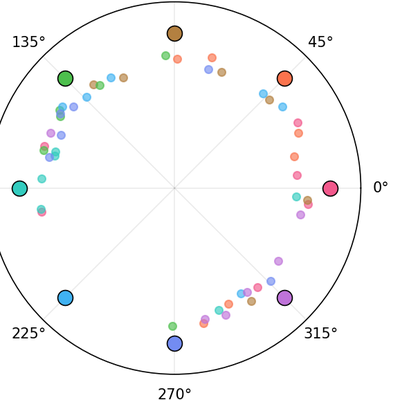
\includegraphics[width=2.5cm,height=2.5cm]{cropped_clean/clean_cvd_V3.png}} \\
\hline
\multirow{2}{*}{\textbf{hV4}} & \textbf{HC} & 82.1° (SD 4.6°) & 27.5 (SD 1.5) & \adjustbox{valign=c}{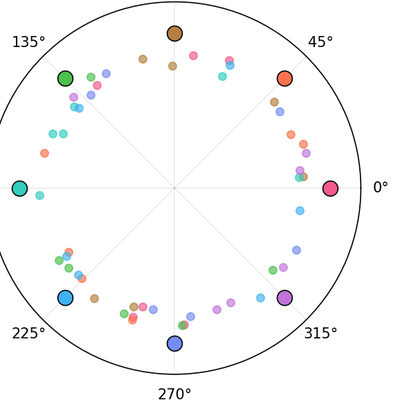
\includegraphics[width=2.5cm,height=2.5cm]{cropped_clean/clean_noncvd_hV4.png}} \\
\cline{2-5}
 & \textbf{CVD} & 76.3° (SD 3.9°) & 29.6 (SD 1.5) & \adjustbox{valign=c}{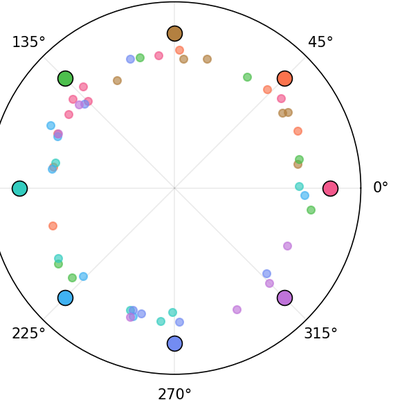
\includegraphics[width=2.5cm,height=2.5cm]{cropped_clean/clean_cvd_hV4.png}} \\
\hline

\end{tabular}
\begin{flushleft}
\scriptsize
\textit{Note: ANOVA config32\_determin analysis results. HC examples from Sub-06; CVD examples from Sub-08.}\\
\textit{Example images show pure circular reconstruction plots (all text removed).}
\end{flushleft}
\end{table}

\clearpage

% Table 2: K5 Permutation Validation Results
\begin{table}[htbp]
\centering
\caption{K5 Permutation Validation Results (k=5 ANOVA Feature Selection)}
\label{tab:k5_permutation}
\large
\renewcommand{\arraystretch}{1.3}
\begin{tabular}{|c|c|c|c|c|c|}
\hline
\rowcolor{green!30}
\textbf{Group} & \textbf{Before Permu} & \textbf{After Permu} & \textbf{Error Change} & \textbf{Effect Size (d)} & \textbf{p-value} \\
\hline
\hline
\textbf{HC} & 78.0° & 81.9° & +3.86° & 0.27 & \textcolor{blue}{\textbf{0.031*}} \\
\hline
\textbf{CVD} & 79.0° & 83.7° & +4.70° & 0.42 & \textcolor{green!60!black}{\textbf{0.011*}} \\
\hline
\end{tabular}
\begin{flushleft}
\small
\textit{* p < 0.05 (significant)}\\
\textit{Note: Both groups show significant validation (p < 0.05), indicating that the k=5 ANOVA}\\
\textit{feature selection successfully identifies informative voxels beyond chance.}
\end{flushleft}
\end{table}

\end{document}
